% Chapter 2
\chapter{From Structured Light to 3D Scanner Calibration based on Pinhole Model} % Main chapter title
\label{sens_PinHoleCameraStructuredLight} % For referencing the chapter elsewhere, use \ref{sens_introduction} 
Pinhole camera model is wildly used in 3D camera's reconstruction, however, it is not able to handle non-linear radial distortion. In this chapter, a pinhole model based 3D camera calibration method (derived from a 3D reconstruction example of structured light method) will be discussed in detail, and then extended into two newly proposed calibration methods.

%%%%%%%%%%%%%%%%%%%%%%%%%%%%%%%%%%%%%%%%%%%%%%%%%%%%%
%%%%%%%%%%                                                     %%%%%%%%%%%%%%%%%%%%%%%%%%
%%%%%%%%%% 2.1   Pinhole Camera Model                   %%%%%%%%%%%%%%%%%%%%%%%%
%%%%%%%%%%                                                     %%%%%%%%%%%%%%%%%%%%%%%%
%%%%%%%%%%%%%%%%%%%%%%%%%%%%%%%%%%%%%%%%%%%%%%%%%%%%%%

\section{Pinhole Camera Model}
\label{sectionPinholeCamera}
%%
Figure \ref{PinholeCameraModel} shows the basic diagram of a pinhole camera model \cite{Maria10} \cite{Zhengyou04} with a reflected image plane for friendly intuition. From this model, the mapping between 3D space world coordinate and the image plane row and column could be separated into two parts of transformations. The first part is the transformation between world coordinates system \(X\)/\(Y\)/\(Z\) and camera coordinate system \(U\)/\(V\)/\(W\) , which forms a 4x4 perspective transformation matrix (\textbf{extrinsic calibration}) that works for 3D rotation and translation. And the second part is the mapping between 3D camera coordinates system \(U\)/\(V\)/\(W\) and 2D image plane coordinates \(u\)/\(v\), which forms a 3x3 perspective transformation matrix (\textbf{intrinsic calibration}) that works for not only the rescaling between camera coordinates and virtual ideal image coordinates, but also for translating and skewing between the virtual ideal image plane and real image plane. %
%
\begin{figure}[h]
\centering
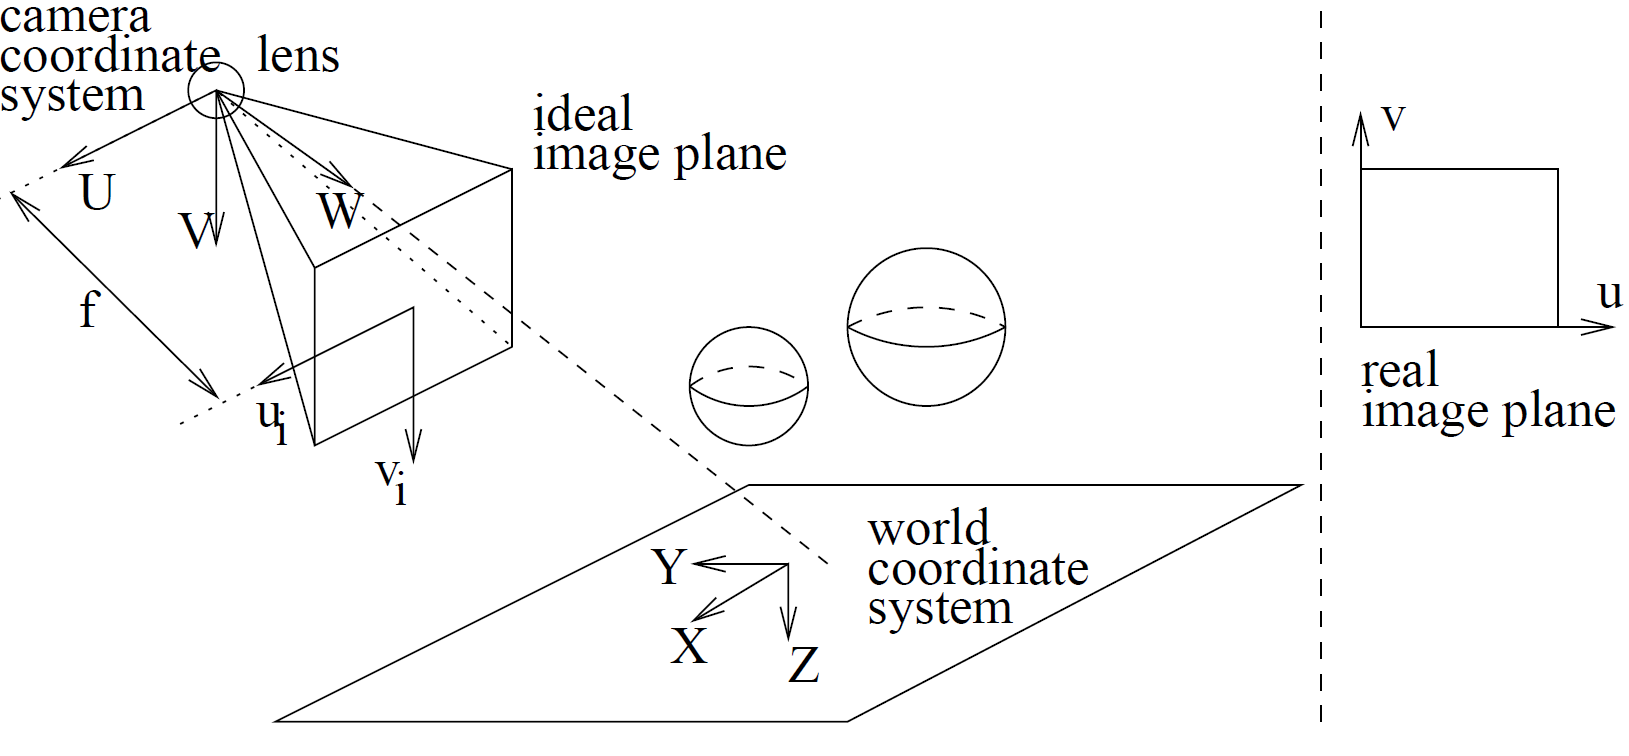
\includegraphics[width=\textwidth]{PinholeCameraModel}
\caption{The pinhole camera model}
\label{PinholeCameraModel}
\end{figure}%
%
\\\par%
\textbf{Extrinsic Calibration}\\
Without any camera parameters, the extrinsic calibration formula could be written, through homogeneous coordinates, as

\begin{equation}
%
\left[ \begin{array}{c} U \\ V \\ W \\ 1 \end{array} \right] %
= %
\begin{bmatrix} R & T \\ 0 & 1 \end{bmatrix} \times \left[ \begin{array}{c} X^w \\ Y^w \\ Z^w \\ 1 \end{array} \right]
%
\end{equation}%
%
or for simplicity,
\begin{equation}
%
\left[ \begin{array}{c} U \\ V \\ W \end{array} \right] %
= %
\begin{bmatrix} R & T \end{bmatrix} \cdot \left[ \begin{array}{c} X^w \\ Y^w \\ Z^w \end{array} \right]
\label{extrinsicTransform}
%
\end{equation}%
%
where \((U, V, W)^T\) are the camera coordinates, and the transformation matrix component \([R\)  \(T]\), which is part of the 4x4 perspective matrix, is modelling rotation and translation , written as

\begin{equation}
%
\left[ \begin{array}{cc} R & T \end{array} \right] %
= %
\begin{bmatrix}
 r_{11} & r_{12} & r_{13} & t_1 \\
 r_{21} & r_{22} & r_{23} & t_2 \\
 r_{31} & r_{32} & r_{33} & t_3
\end{bmatrix}
%
\end{equation}
\\\par
%
%
\textbf{Intrinsic Calibration}\\
Intrinsic Calibration could be separated into two sections. The first section is to rescale from camera coordinates to virtual ideal image coordinates. For a easier integration of two sections, the first section's formula is given through both of 2D coordinates to homogeneous coordinates.\par
%
\quad\quad2D coordinates:%
\begin{equation}
%
W \left[ \begin{array}{c} u_i \\ v_i  \end{array} \right] %
= f %
\left[ \begin{array}{c} U \\ V \end{array} \right]%
%
\end{equation}

\quad\quad Homogeneous coordinates:\par
\begin{equation}
%
W \left[ \begin{array}{c} u_i \\ v_i \\ 1 \end{array} \right] %
= %
\left[ \begin{array}{c} fU \\ fV \\ W \end{array} \right]%
=  \begin{bmatrix} f & 0 & 0 \\ 0 & f & 0 \\ 0 & 0 & 1 \end{bmatrix} \cdot %
\left[ \begin{array}{c} U \\ V \\ W \end{array} \right]%
\label{section_1}
\end{equation}%
\\\par
%
The second section is for translating and skewing between the virtual ideal image plane \(u_i\)/\(v_i\) and real image plane \(u_r\)/\(v_r\),  %

\begin{equation}
%
\left[ \begin{array}{c} u_r \\ v_r \\ 1 \end{array} \right] %
=  \begin{bmatrix} s_u & s_\theta & u_0 \\ 0 & s_v & v_0 \\ 0 & 0 & 1 \end{bmatrix} \cdot %
\left[ \begin{array}{c} u_i \\ v_i \\ 1 \end{array} \right]%
\label{section_2}
\end{equation}%
where \((u_0, v_0)\) denotes the optical center (or principal point), \([s_u, s_v]\) are skew coefficients in pixels along \(u\) and  \(v\) axes , and  \(s_\theta\) is an skewed angle generated by \(s_u\) and  \(s_v\). To combine equation \ref{section_1} and equation \ref{section_2}, we could get %

\begin{equation}
%
W \left[ \begin{array}{c} u_r \\ v_r \\ 1 \end{array} \right] %
=  \begin{bmatrix} s_u & s_\theta & u_0 \\ 0 & s_v & v_0 \\ 0 & 0 & 1 \end{bmatrix} \cdot%
 \begin{bmatrix} f & 0 & 0 \\ 0 & f & 0 \\ 0 & 0 & 1 \end{bmatrix} \cdot %
\left[ \begin{array}{c} U \\ V \\ W \end{array} \right]%
=  \begin{bmatrix} f_u & s & u_0 \\ 0 & f_v & v_0 \\ 0 & 0 & 1 \end{bmatrix} \cdot%
\left[ \begin{array}{c} U \\ V \\ W \end{array} \right]%
%
\label{intrinsicTransform}
\end{equation}%
%
where \([f_u,\, f_v]\) denote focal lengths in pixels along \(u\) and \(v\) after skewing, and \(s\) is a new skew coefficient after combination.\\\par%
%
\textbf{Generic Perspective Matrix of the Pinhole Camera Model}\par%
\noindent
After both of the extrinsic and intrinsic transformation matrices have been derived, the generalization formula of the pinhole camera model could be derived, combining equation \ref{extrinsicTransform} and \ref{intrinsicTransform}, as

\begin{equation}
%
k \left[ \begin{array}{c} u_r \\ v_r \\ 1 \end{array} \right] %
=  \begin{bmatrix} f_u & s & u_0 \\ 0 & f_v & v_0 \\ 0 & 0 & 1 \end{bmatrix} \cdot%
\begin{bmatrix} R & T \end{bmatrix} \cdot \left[ \begin{array}{c} X^w \\ Y^w \\ Z^w \end{array} \right]%
=  C \cdot \left[ \begin{array}{c} X^w \\ Y^w \\ Z^w \end{array} \right]%
%
\label{detailedPerspectivePinholeCameraMatrix}
\end{equation}%
%
where \(W\) on the left side has been replaced by \(k\) to be a more general proportion coefficient, and a combined matrix can be expressed as
\begin{equation}
%
C %
=  \begin{bmatrix} f_u & s & u_0 \\ 0 & f_v & v_0 \\ 0 & 0 & 1 \end{bmatrix} \cdot%
\begin{bmatrix} R & T \end{bmatrix}%
= \begin{bmatrix} 
m_{11} & m_{12} & m_{13} & m_{14} \\
m_{21} & m_{22} & m_{23} & m_{24} \\
m_{31} & m_{32} & m_{33} & m_{34} \\
\end{bmatrix}%
%
\label{genericPerspectivePinholeMatrix}
\end{equation}%
%
The final 3x4 matrix C is considered as the generic perspective transformation matrix of a pinhole camera model, which gives a mapping between the 3D world coordinates and 2D real image coordinates. To inspect the pinhole camera matrix, its effects focuses on the linear processes of rotation and translation, given a perspective view. In other words, this 3x4 transformation matrix is specially for perspective distortion removal. It is built on the homogeneous coordinates, which is built on, and also limited by the linear system. And a mapping using this 3x4 transformation matrix between two coordinates can only be linear (handle linear perspective distortion).\par


%%%%%%%%%%%%%%%%%%%%%%%%%%%%%%%%%%%%%%%%%%%%%%%%%%%%%%%
%%%%%%%%%%                                                                              %%%%%%%%%%%%%%%%%%%%%
%%%%%%%%%% 2.2   Structured Light 3D Reconstruction in Real-Time   %%%%%%%%%%%%%%%%%%%
%%%%%%%%%%                                                                                 %%%%%%%%%%%%%
%%%%%%%%%%%%%%%%%%%%%%%%%%%%%%%%%%%%%%%%%%%%%%%%%%%%%
\section{Structured Light 3D Reconstruction in Real-Time}
\label{sectionSL3DReconstructionRealTime}
Using a 3D reconstruction method of structured light, applying Phase Measuring Profilometry (PMP) technique, a per-pixel 3D camera calibration method based on pinhole camera model is detailedly introduced in this section. Both of the advantage and disadvantage are discussed.
%
%
\begin{figure}[H]
\centering
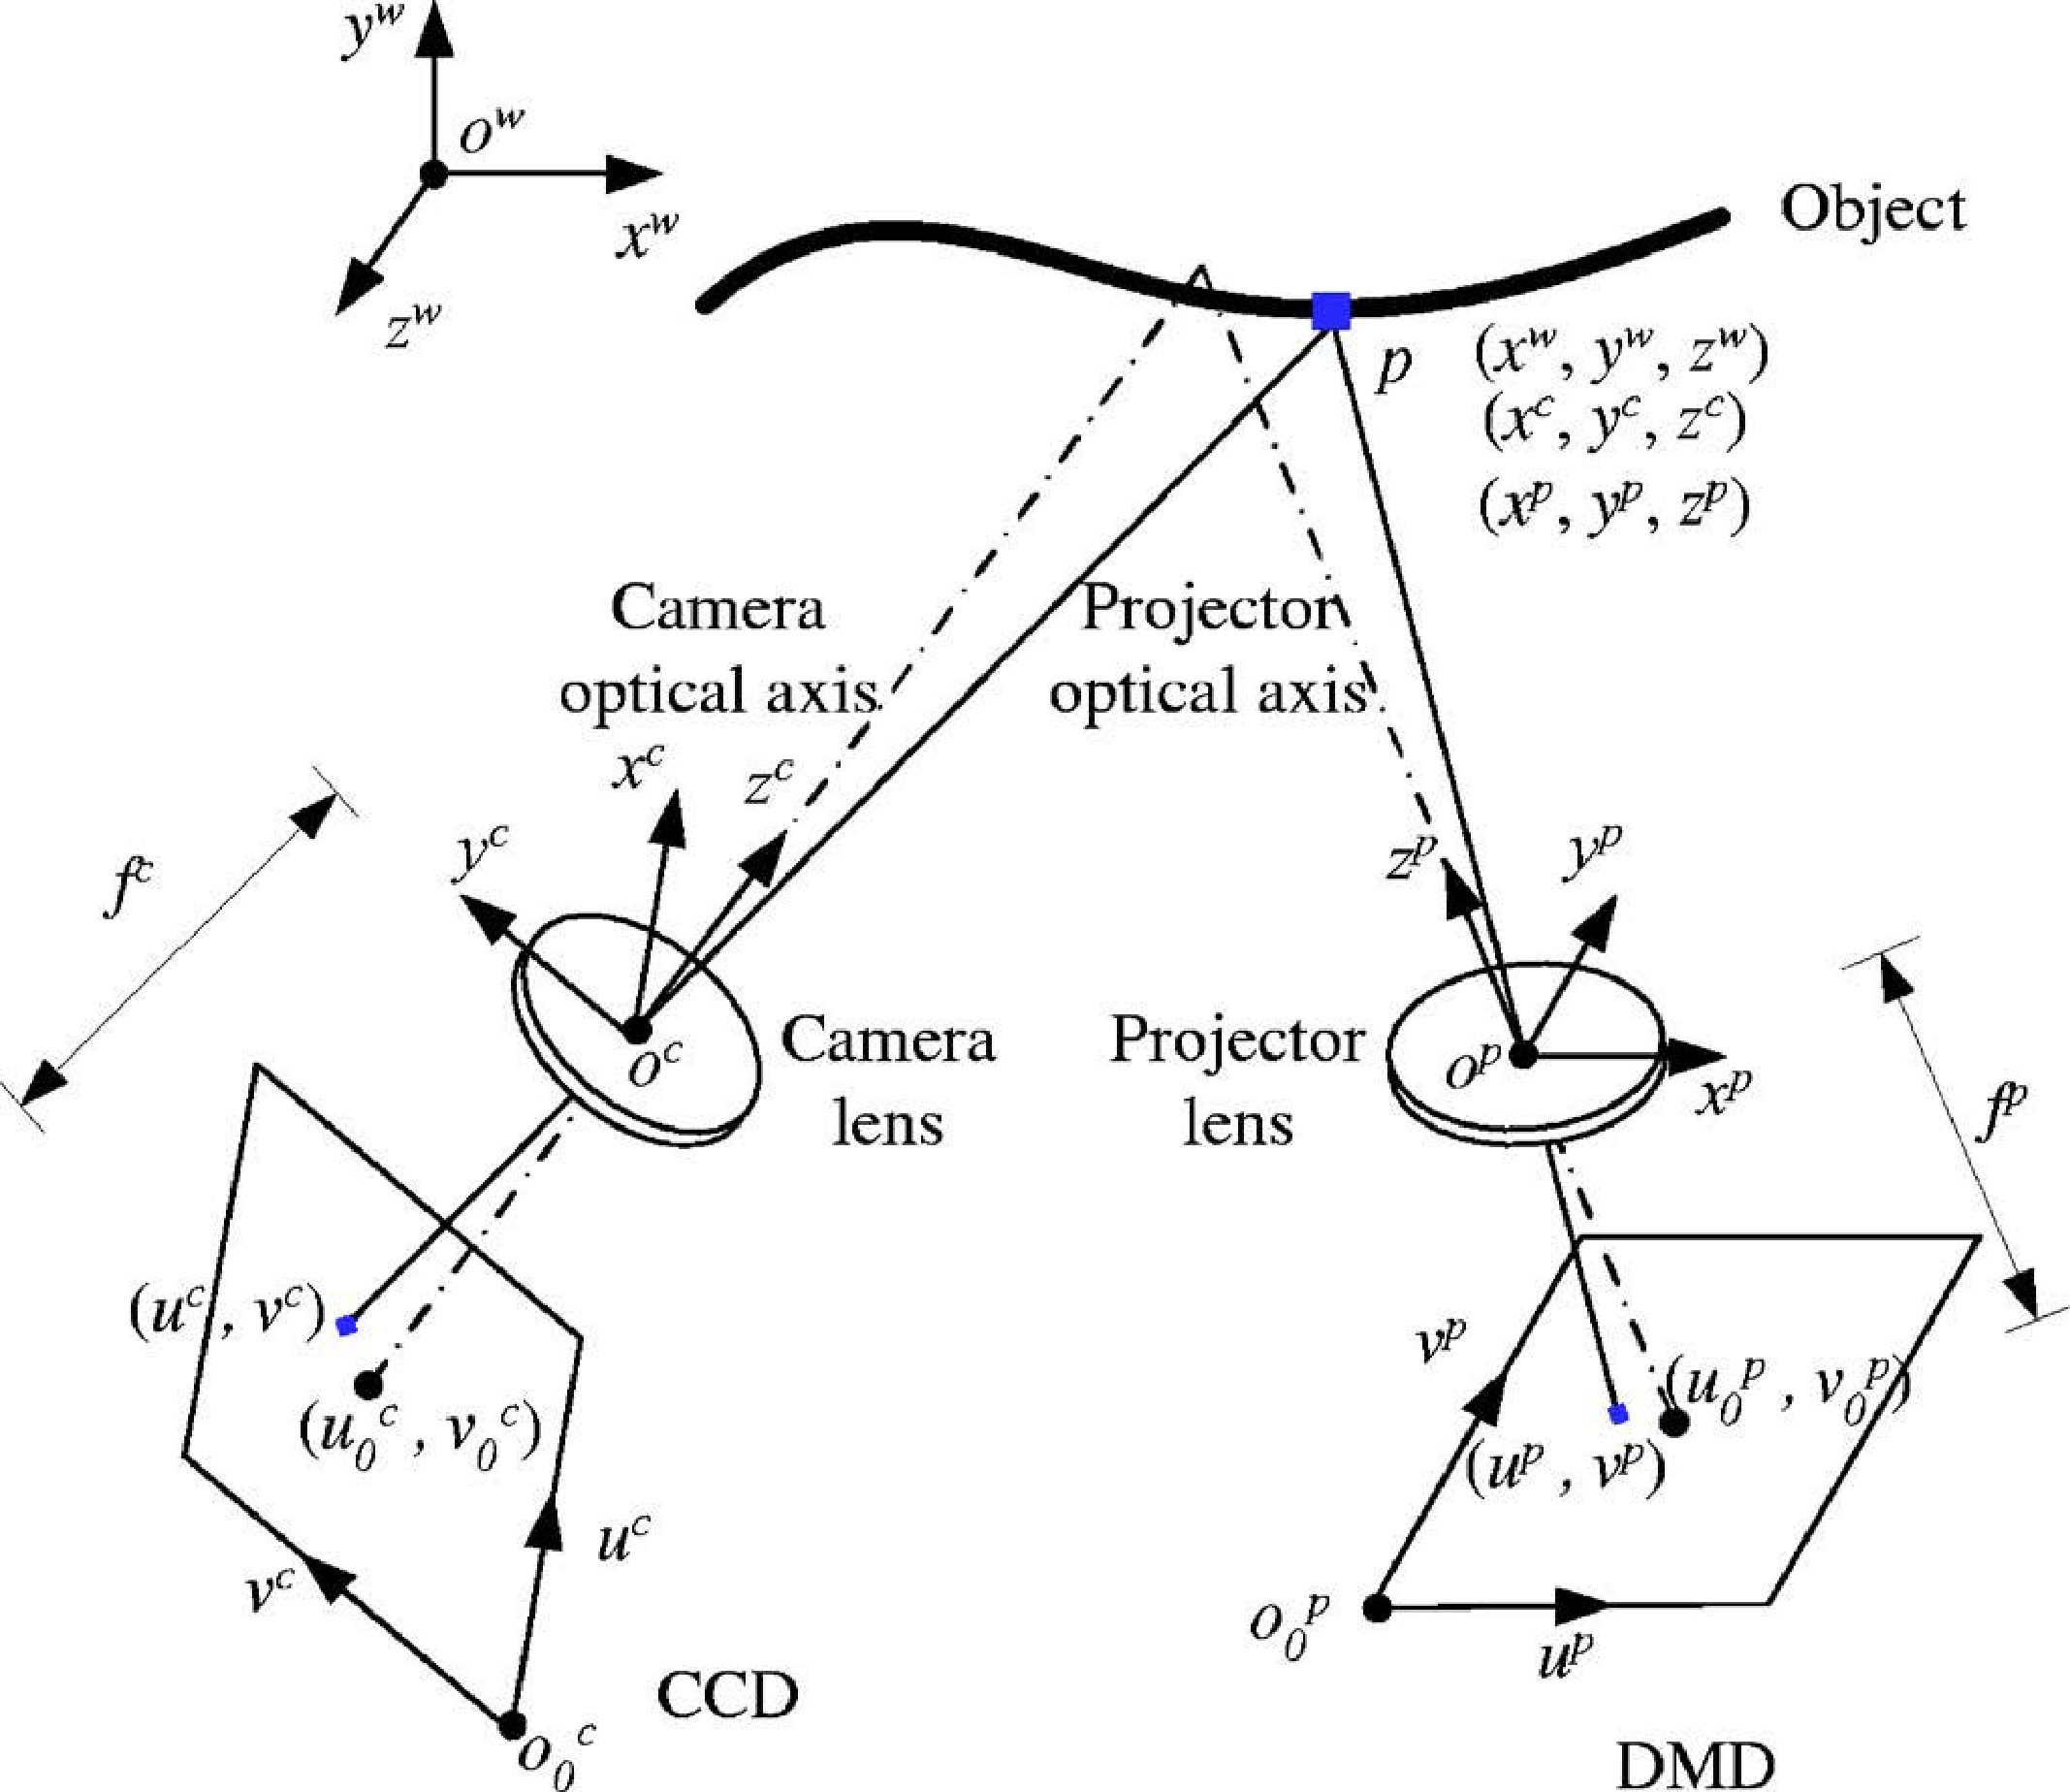
\includegraphics[width=0.7\textwidth]{SLPMPConfiguration}
\caption{SL PMP Configuration Diagram \cite{Song06}}
\label{SLPMPConfiguration}
\end{figure}%
%
A 3D shape measurement system consists of a Charge-Coupled Device (CCD) camera and a Digital Micro-mirror Device (DMD) projector. 2D image pattern strategies are always preferred for fast scanning if a DMD projector is involved
[**]%J. Salvi, J. Pages, and J. Batlle, \Pattern codication strategies in structured light systems," Pattern Recognition 37, 827{849 (2004).
 \cite{Song06}.
And the multi-shot pattern Phase Measuring Profilometry strategy was used for its properties of robust and accuracy.
With PMP information encoded in the structured light pattern projected onto the target, the CCD camera could capture a series of images that contains PMP informatio. Triangulation analyzing could be used to extract the 3D world coordinates for each points of the target profile, by a determination of the relationships among CCD camera, DMD projector, and the target object. A system configuration of PMP application is given in figure \ref{SLPMPConfiguration}.%
\\\\%
PMP method uses either vertical or horizontal sinusoid patterns, which could be described as:

 \begin{equation}
%
I^p_n(x^p, \, y^p) %
= A^p(x^p, \, y^p) + B^p(x^p, \, y^p)Cos(2\pi fy^p - \frac{2\pi n}{N})
%
\end{equation}%
%
where \((x^p, \, y^p)\) denotes the coordinates of every single pixel in the projector, \(I^p_n\) denotes the intensity of the corresponding pixels, \(A^p\) and \(B^p\) are constants, \(f\) is the frequency of sine wave. The subscript \(n\) represents the index of phase shift, while capital \(N\) is the total number of phase shift.\par%
%
%
 \begin{figure}[h]
%\centering
\hspace*{-2cm} 
\subfloat[Pattern 0][1]{

\includegraphics[width=0.3\textwidth]{Pattern0}
\label{fig:subfig1}}
\subfloat[Pattern 1][2]{

\includegraphics[width=0.3\textwidth]{Pattern1}
\label{fig:subfig2}}
\subfloat[Pattern 2][3]{

\includegraphics[width=0.3\textwidth]{Pattern2}
\label{fig:subfig3}}
%\qquad
\subfloat[Pattern 3][4]{

\includegraphics[width=0.3\textwidth]{Pattern3}
\label{fig:subfig4}}
\caption{PMP base frequency patterns}
\label{PMPFrequencyPatterns}
\end{figure}%
%
%\begin{figure}
%    \centering
%    \hspace*{-3cm} 
%    \begin{subfigure}[b]{0.3\textwidth}
%            
\includegraphics[width=\textwidth]{Pattern0}
%            \caption{Pattern 0}
%    \end{subfigure}%
%    ~ 
%    \begin{subfigure}[b]{0.3\textwidth}
%            
\includegraphics[width=\textwidth]{Pattern1}
%            \caption{Pattern 1}
%    \end{subfigure}
%    ~ 
%    \begin{subfigure}[b]{0.3\textwidth}
%            
\includegraphics[width=\textwidth]{Pattern2}
%            \caption{Pattern 2}
%    \end{subfigure}
%    ~ 
%    \begin{subfigure}[b]{0.3\textwidth}
%            
\includegraphics[width=\textwidth]{Pattern3}
%            \caption{Pattern 3}
%    \end{subfigure}
%    \caption{PMP base frequency patterns}
%    \label{PMPFrequencyPatterns}
%\end{figure}
%
%
%
Figure \ref{PMPFrequencyPatterns} shows a group of sine wave patterns, where the number of total phase shift \(N = 4\) and frequency \(f = 1\). From viewpoint of the camera, the sinusoid patterns is distorted by the target surface topology, so that the captured images could be expressed as 

 \begin{equation}
%
I^c_n(x^c, \, y^c) %
= A^c(x^c, \, y^c) + B^c(x^c, \, y^c)Cos[\phi(x^c,\, y^c) - \frac{2\pi n}{N}]
%
\end{equation}%
%
where\((x^c, \, y^c)\) denotes the coordinates of every single pixel in the camera, and the term \(\phi(x^c,\, y^c)\) represents the corresponding phase value, which could be computed as follows [6]\par
 % Very High Resolution 3-D surface Scanning Using Multi-Frequency Phase Measuring Profilometry
 \begin{equation}
%
\phi(x^c,\, y^c) %
= arctan\Bigg[\frac{\sum^N_{n=1}I(x^c,\,y^c)Sin(2\pi n / N)}{\sum^N_{n=1}I(x^c,\,y^c)Cos(2\pi n / N)} \Bigg]
%
\label{equationArctangent}
\end{equation}
%
%
After the camera term  \(\phi(x^c,\, y^c)\)  for every single pixel is computed, the corresponding projector coordinate \(y^p\) could be derived through equation\par

\begin{equation}
%
y^p %
= \phi(x^c,\, y^c) / (2\pi f)
%
\end{equation}%
%
With the knowledge of \(y^p\), the perspective information between camera and projector is the last step to go for applying triangulation analysis to extract world coordinates. Based on pinhole camera model, the perspective matrices for both of the CCD camera and DMD projector, as will be derived later in section \ref{sectionPinholeCamera} equation \ref{genericPerspectivePinholeMatrix}, are written as [7]\par
% J. Li, L. G. Hassebrook, and C. Guan, \Optimized two-frequency phasemeasuring-prolometry light-sensor temporal-noise sensitivity," Journal of the Optical Society of America A 20, 106{115 (2003).

\begin{equation}
%
M^c %
= \begin{bmatrix} 
m^c_{11} & m^c_{12} & m^c_{13} & m^c_{14} \\
m^c_{21} & m^c_{22} & m^c_{23} & m^c_{24} \\
m^c_{31} & m^c_{32} & m^c_{33} & m^c_{34} \\
\end{bmatrix}%
%
%\label{genericPerspectivePinholeMatrix}
\end{equation}%
%
and 

\begin{equation}
%
M^p %
= \begin{bmatrix} 
m^p_{11} & m^p_{12} & m^p_{13} & m^p_{14} \\
m^p_{21} & m^p_{22} & m^p_{23} & m^p_{24} \\
m^p_{31} & m^p_{32} & m^p_{33} & m^p_{34} \\
\end{bmatrix}%
%
%\label{genericPerspectivePinholeMatrix}
\end{equation}%
%
The mapping from 3D world coordinates to 2D camera coordinates are given by\par

\begin{equation}
%
x^c %
= \frac%
{m^c_{11}X^w + m^c_{12}Y^w + m^c_{13}Z^w + m^c_{14}}%
{m^c_{31}X^w + m^c_{32}Y^w + m^c_{33}Z^w + m^c_{34}}
%
\label{cameraXmapping}
\end{equation}%
%
%
\begin{equation}
%
y^c %
= \frac%
{m^c_{21}X^w + m^c_{22}Y^w + m^c_{23}Z^w + m^c_{24}}%
{m^c_{31}X^w + m^c_{32}Y^w + m^c_{33}Z^w + m^c_{34}}
%
\label{cameraYmapping}
\end{equation}%
%
%
Likewise, the translation from 3D world coordinates to 2D projector coordinates are given by\par
\begin{equation}
%
x^p %
= \frac%
{m^p_{11}X^w + m^p_{12}Y^w + m^p_{13}Z^w + m^p_{14}}%
{m^p_{31}X^w + m^p_{32}Y^w + m^p_{33}Z^w + m^p_{34}}
%
\label{projectorXmapping}
\end{equation}%
%
\begin{equation}
%
y^p %
= \frac%
{m^p_{21}X^w + m^p_{22}Y^w + m^p_{23}Z^w + m^p_{24}}%
{m^p_{31}X^w + m^p_{32}Y^w + m^p_{33}Z^w + m^p_{34}}
%
\label{projectorYmapping}
\end{equation}%
%
%
Since three out of four equations \ref{cameraXmapping} \texttildelow \,\ref{projectorYmapping} are enough to solve \(X^{w}\),  \(Y^{w}\),  and \(Z^{w}\), and \(y^p\) is already calculated, the 3D world coordinates \(X^{w}\)/\(Y^{w}\)/\(Z^{w}\)  could be derived from Eqs  \ref{cameraXmapping},  \ref{cameraYmapping}, and \ref{projectorYmapping}\par%
%
\begin{equation}
\hspace*{-0.3cm} 
%
\left[ \begin{array}{c} X^w\\ Y^w\\ Z^w\end{array} \right] %
= %
\begin{bmatrix} %
m^c_{11} - m^c_{31}x^c, &m^c_{12} - m^c_{32}x^c, &m^c_{13} - m^c_{33}x^c \\%
m^c_{21} - m^c_{31}y^c, &m^c_{22} - m^c_{32}y^c, &m^c_{23} - m^c_{33}y^c \\%
m^p_{21} - m^p_{31}y^p, &m^p_{22} - m^p_{32}y^p, &m^p_{23} - m^p_{33}y^p %
\end{bmatrix} ^{-1} %
\left[ \begin{array}{c}%
m^c_{34}y^c - m^c_{14}\\%
m^c_{34}y^c - m^c_{24}\\%
m^p_{34}y^p - m^p_{24}%
\end{array} \right]
%
\label{equationInversion}
\end{equation}%
\\\\%
%
\noindent
Traditionally, as derived above, it is the arctangent computation (equation \ref{equationArctangent}) and the matrix inversion (equation \ref{equationInversion}) that prove to be the bottleneck, preventing real-time surface reconstruction. However, Kai proposed a LUT-based solution that solves the bottleneck by expanding those two equations into new forms, directly building accurate LUTs. Based on Kai's derivation \cite{Kai10}, \(X^{w}\) and \(Y^{w}\) can be computed respectively as 
%
\begin{equation}
X^w_{(col^c, \, row^c)} = c_{(col^c, row^c)}Z^w_{(col^c, \, row^c)}+d_{(col^c, row^c)}
\label{equationLUT_X}
\end{equation}%
and %
\begin{equation}
Y^w_{(col^c, \, row^c)} = e_{(col^c, row^c)}Z^w_{(col^c, \, row^c)}+f_{(col^c, row^c)}
\label{equationLUT_Y}
\end{equation}
%
where 
%
\begin{equation*}%
c_{(col^c, row^c)} %
= \frac%
{(m^c_{22}m^c_{33} - m^c_{23}m^c_{32})col^c + (m^c_{13}m^c_{32} - m^c_{12}m^c_{33})row^c + (m^c_{12}m^c_{23} - m^c_{13}m^c_{22})}%
{(m^c_{21}m^c_{32} - m^c_{22}m^c_{31})col^c + (m^c_{12}m^c_{31} - m^c_{11}m^c_{32})row^c + (m^c_{11}m^c_{22} - m^c_{12}m^c_{21})} \, ,
\end{equation*}
%
\begin{equation*}%
d_{(col^c, row^c)} %
= \frac%
{(m^c_{22}m^c_{34} - m^c_{24}m^c_{32})col^c + (m^c_{14}m^c_{32} - m^c_{12}m^c_{34})row^c + (m^c_{12}m^c_{24} - m^c_{14}m^c_{22})}%
{(m^c_{21}m^c_{32} - m^c_{22}m^c_{31})col^c + (m^c_{12}m^c_{31} - m^c_{11}m^c_{32})row^c + (m^c_{11}m^c_{22} - m^c_{12}m^c_{21})} \, ,
\end{equation*}
%
\begin{equation*}%
e_{(col^c, row^c)} %
= \frac%
{(m^c_{23}m^c_{31} - m^c_{21}m^c_{33})col^c + (m^c_{11}m^c_{33} - m^c_{13}m^c_{31})row^c + (m^c_{13}m^c_{21} - m^c_{11}m^c_{23})}%
{(m^c_{21}m^c_{32} - m^c_{22}m^c_{31})col^c + (m^c_{12}m^c_{31} - m^c_{11}m^c_{32})row^c + (m^c_{11}m^c_{22} - m^c_{12}m^c_{21})} \, ,
\end{equation*}
%
\begin{equation*}%
f_{(col^c, row^c)} %
= \frac%
{(m^c_{23}m^c_{32} - m^c_{22}m^c_{33})col^c + (m^c_{12}m^c_{33} - m^c_{13}m^c_{32})row^c + (m^c_{13}m^c_{22} - m^c_{12}m^c_{23})}%
{(m^c_{21}m^c_{32} - m^c_{22}m^c_{31})col^c + (m^c_{12}m^c_{31} - m^c_{11}m^c_{32})row^c + (m^c_{11}m^c_{22} - m^c_{12}m^c_{21})}
\end{equation*}
%
and (\(col^c, \, row^c\)) denote the address of a camera's pixel, \(c\)/\(d\)/\(e\)/\(f\) are the corresponding linear coefficients that help map from \(Z^w\) to \(X^w\) and \(Y^w\).%
\\\\%
After Kai's expansion from equation equation \ref{equationInversion} to equation \ref{equationLUT_X} and \ref{equationLUT_Y}, the parameters of the projector's pinhole camera matrix are gone, and everything left belongs to the camera (with superscript of \(c\)). It means that, for arbitrary RGB-D 3D camera, its calibration could be done by acquiring its 3-by-4 pinhole camera matrix, and then generating beam equations of \ref{equationInversion} and \ref{equationLUT_X} for every single pixel.
%
%%%%%%%%%%%%%%%%%%%%%%%%%%%%%%%%%%%%%%%%%%%%%%%%%
%%%%%%%%%%                                                                       %%%%%%%%%%%%%
%%%%%%%%%%        3.3  Shortcoming and Extension                  %%%%%%%%%%%%%%%%%%%
%%%%%%%%%%                                                                                 %%%%%%%%%%%%%
%%%%%%%%%%%%%%%%%%%%%%%%%%%%%%%%%%%%%%%%%%%%%%%%%%%%%
\section{Shortcoming and Extension}
\subsection{Shortcoming}
The camera calibration method discussed in section \ref{sectionSL3DReconstructionRealTime} is totally derived from the pinhole camera model, which gives the relationship from \(Z^w\) to \(X^w\) and \(Y^w\), and the 2D mapping from \(u_r\)/\(v_r\) (\(column\)/\(row\)) to \(X^w\)/\(Y^w\), as figure \ref{PinholeCameraModel} shows. And equation \ref{genericPerspectivePinholeMatrix} and \ref{detailedPerspectivePinholeCameraMatrix} tell us that, the pinhole matrix can only handle linear transformation, i.e., the calibration exclusively based on the pinhole camera model can only handle perspective distortions, whereas the most important radial dominated non-linear lens distortions still exist inside \(X^w\) and \(Y^w\).%
%
\\\\%
Lens distortion could be classified into two groups [10] : radial distortion, and tangential distortion.\par
%Z. Zhang, "Camera Calibration",   Chapter 2, pages 4-43, in G. Medioni and S.B. Kang, eds., Emergin Topics in Computer Vision, Prentice Hall Professional Technical Reference, 2004. .\par
%
Imperfect lens shape causes light rays bending more near the edges of a lens than they do at its optical center. The smaller the lens, the greater the distortion. Barrel distortions happen commonly on wide angle lenses, where the field of view of the lens is much wider than the size of the image sensor.\par%
Improper lens assembly will lead to tangential distortion, which occurs when the lens and the image plane are not parallel.\par%
%
%
Figure \ref{NIR_by_Depth_front} shows the front view of raw NearIR steam 3D reconstruction, with a blue rectangle along the outermost layer of dot-clusters near the border. Due to the radial dominated distortions, most of the dot-clusters on the outermost layer are not sitting on the four sides (straight lines) of the rectangle.\\\\
%
The lens distortion can be expressed as power series in radial distance \(r = \sqrt{x^2 + y^2}\):
\begin{equation}
%
\begin{aligned}
x_{distorted} =  x (1 + k_1 r^2 + k_2 r^4 + k_3 r^6) + [p_1 (r^2 + 2 x^2) + 2 p_2 xy] %
\\%
y_{distorted} =  y (1 + k_1 r^2 + k_2 r^4 + k_3 r^6) + [p_2 (r^2 + 2 y^2) + 2 p_1 xy]
\end{aligned}
\label{lensDistortion}
%
\end{equation}%
%
where higher order parameters are omitted for being negligible; \((x_{distorted}, \, y_{distorted})\) denote the distorted points, \((x, \, y)\) denote the undistorted pixel locations, \(k_i\)'s are coefficients of radial distortion, and \(p_j\)'s are coefficients of tangential distortion.%
%
%
Equation \ref{lensDistortion} tells us that, high order polynomial mapping is needed in order to remove the lens distortions. However, the 3-by-4 camera matrix is fixed by order \(1st\) (linear) that, it is impossible to make \(X^w\)/\(Y^w\) be mapped from \(column\) / \(row\) by a higher order polynomial transformation. We have to relinquish the pinhole model's benefit of 2D mapping from \(column\) / \(row\) to \(X^w\)/\(Y^w\), and have to relinquish equation  \ref{equationInversion}, \ref{equationLUT_X} and \ref{equationLUT_Y}.%
%
%%%%%%%%%%%%%
%%%%%%%%%%%%%
%%%%%%%%%%%%%
%%%%%%%%%%%%%
\subsection{Extended Method One}
Although the 3-by-4 pinhole camera matrix is not helpful for removing lens distortion, the pinhole camera model is still a good model that can help determining the relationship from \(Z^w\) to \(X^w\) and \(Y^w\), and that is exactly what a 3D camera calibration needs for determining the beam equation for every single pixel.%
\\\\%
Figure \ref{CaliPinHolCameraModel} shows the lens distortion removed pinhole camera model. In this model, the coordinates-pairs (\(column\) / \(row\) and \(X^w\)/\(Y^w\)), which was used to train the 3-by-4 pinhole matrix, are now used to train a high order polynomial transformation matrix. The orange pillow shape shows the lens distortion removed image, which was a rectangle in blue.
%
\begin{figure}[H]
\centering
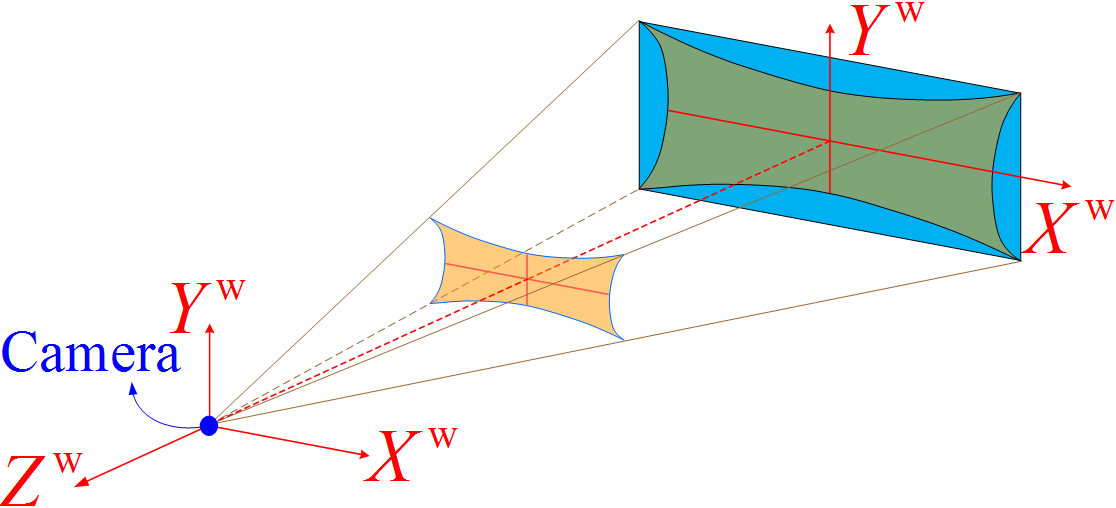
\includegraphics[width=\textwidth]{CaliPinHolCameraModel}
\caption{Lens Distortion Removed Pinhole Camera model}
\label{CaliPinHolCameraModel}
\end{figure}%
%
\noindent
With \(X^w\)/\(Y^w\)'s lens distortions removed, the last thing to go for is to calculate beam equations for every single pixel. It is straight forward to determine a line equation (beam equation) given two know points. The first point is the origin, and the second point could be calculated using the high order transformation matrix.
%%%%%%%%%%%%%
%%%%%%%%%%%%%
%%%%%%%%%%%%%
%%%%%%%%%%%%%
\subsection{Extended Method Two}
The extended method one, which is introduced above, is still not ideal. The focal point and focal length of a camera practically will change as its lens changes, so that light rays should not converge at the origin, and probably not even at one point. In order to get more accurate LUT for a better 3D view, the second point of the beam for every single pixel should also be a datum retrieved from the camera. %
\\\\%
The second method, chasing after accuracy, is to add a rail along \(Z^w\)-axis for multiple points data acquisition. Not only real points (in contrast to assuming the origin as the second point) will be used for beam equation determination, but the \(Z^w\) values could also be calibrated with external accurate data support in case \(depth\) distortion (as shown in figure \ref{NIR_by_Depth_LeftSide}).
%
\begin{figure}[H]
\centering
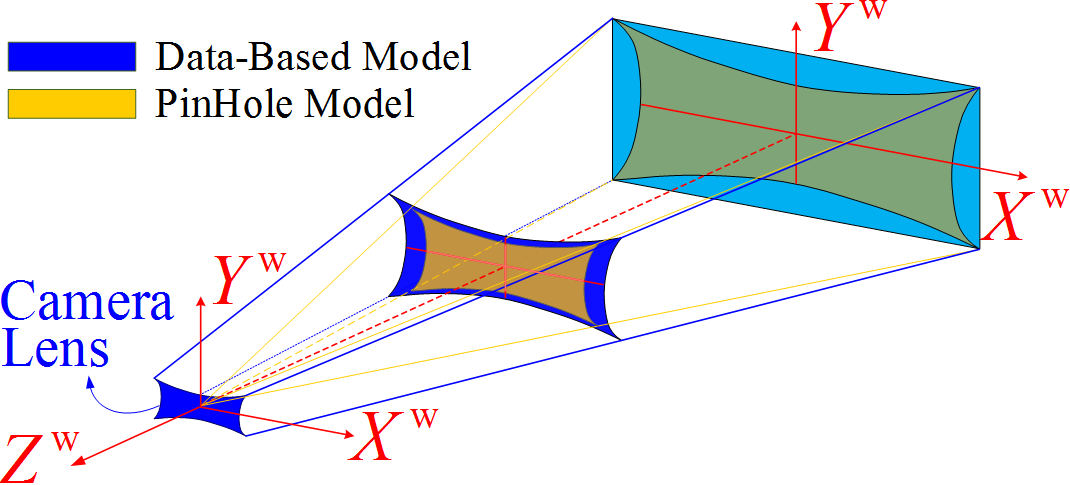
\includegraphics[width=\textwidth]{DataBasedCalibrationModel}
\caption{Comparison: Data-Based Calibration and Pinhole Model Calibration}
\label{DataBasedCalibrationModel}
\end{figure}%
%
%
\noindent
Figure \ref{DataBasedCalibrationModel} gives the data-based model in dark blue, in which the light rays will converge in front of the origin (the lens prolongs the focal length from in front of the origin to the origin) with also a pillow shape. This model is proved practically on KinectV2 in section \ref{finalDataBasedModelReconstruction} figure \ref{SampleBeams_NearIR}.


























